\section{Results} \label{sec:results}

\subsection{Parameter Optimization}

For SVM, we optimized parameter $\gamma$ and found the optimum to be
$\gamma = 0.3$. Changing other parameters from their defaults did not
yield notable improvements. Otherwise, we used the default parameter
values that Weka 3.6.5 provides for LibSVM.

The accuracies of different parameter combinations for the Bernoulli
mixture are shown in Figure (lisää kuva results/bmix\_opt.pdf). The best
accuracy (98.0 \%) was obtained with 12 ham components and 17 spam
components.

\begin{figure}[!ht]
\centering
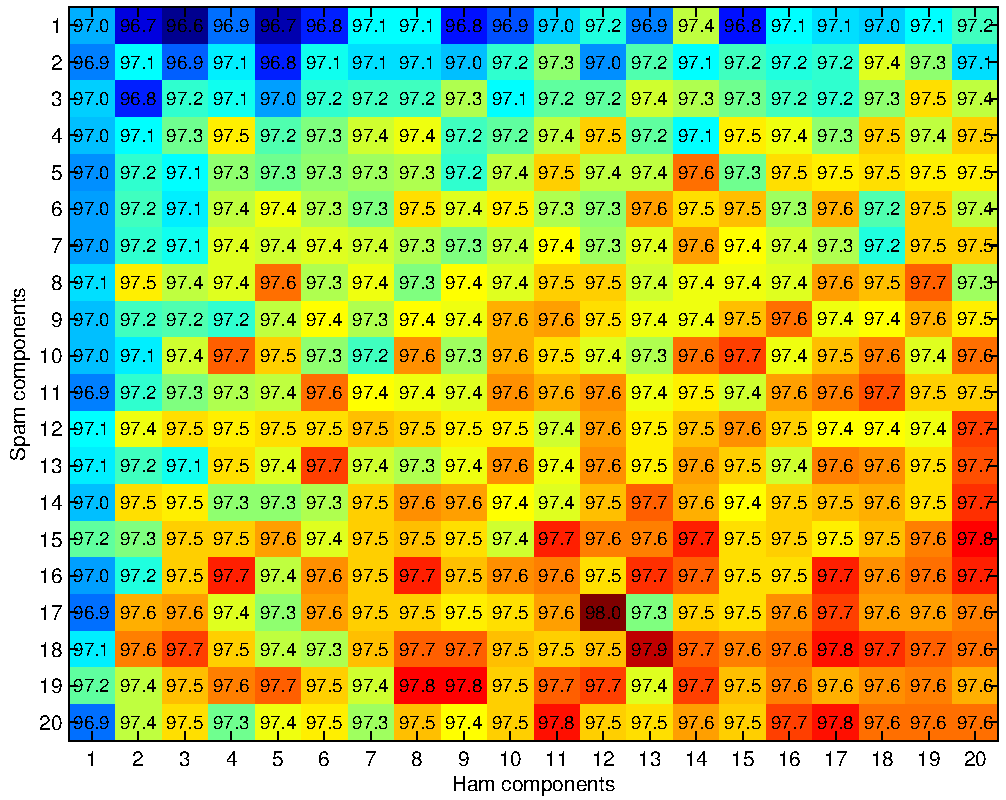
\includegraphics[width=\linewidth]{../results/bmix_opt.pdf}
\caption{Bernoulli mixture accuracies with different number of spam and ham components.}
\label{fig:bmix}
\end{figure}

With the Random Forest classifier, we chose to use the default
parameters as changing these did not seem to affect the classification
accuracy significantly.

\subsection{Classification}

The average cross-validation accuracy of each classifier for the known
data is shown in Table \ref{results1k}.

\begin{table}[!ht]
\caption{Average accuracy on known data (10-fold cross-validation)}
\label{results1k}
\begin{center}
\begin{tabular}{l|c}
Classifier & Accuracy \\ \hline
SVM & 98.4\% \\
Bernoulli mixture & 98.0\% \\
Random forest & 97.1\% \\
\end{tabular}
\end{center}
\end{table}

The ensemble method gave us $99.2 \%$ accuracy with a simple half-half
split of the known data that was used also for the parameter
optimization. Test accuracies and error counts for unknown 9000 data
samples are given in Table \ref{results9k}.

\begin{table}[!ht]
\caption{Accuracy and error count on unknown data}
\label{results9k}
\begin{center}
\begin{tabular}{l|c|c}
Classifier & Accuracy & Error count \\ \hline
SVM & 97.2\% & 251 \\
Bernoulli mixture & 98.0\% & 181 \\
Random forest & 96.3\% & 329 \\ \hline
Ensemble method & 98.0\% & 179 \\
\end{tabular}
\end{center}
\end{table}
